

\tikzset{every picture/.style={line width=0.75pt}} %set default line width to 0.75pt        

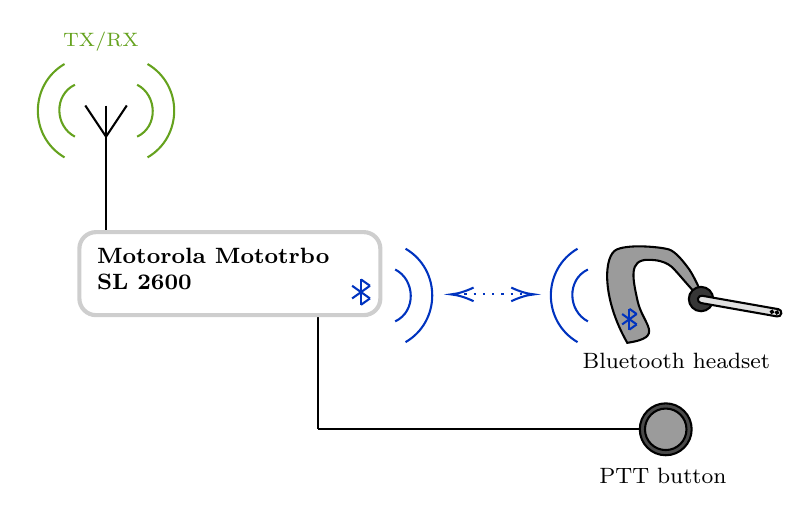
\begin{tikzpicture}[x=0.75pt,y=0.75pt,yscale=-1,xscale=1]
%uncomment if require: \path (0,611); %set diagram left start at 0, and has height of 611

%Straight Lines [id:da6025377414505892] 
\draw    (275,365) -- (275,420) ;
%Straight Lines [id:da8632563010362544] 
\draw    (172.84,264) -- (172.84,324) ;
%Straight Lines [id:da9125480475574657] 
\draw    (162.84,264) -- (172.84,279) ;
%Straight Lines [id:da061481860873287] 
\draw    (172.84,279) -- (182.84,264) ;
%Curve Lines [id:da709923124702297] 
\draw [color={rgb, 255:red, 101; green, 162; blue, 30 }  ,draw opacity=1 ]   (187.84,254) .. controls (197.56,259) and (198.13,274.14) .. (187.84,279) ;
%Curve Lines [id:da449825910233995] 
\draw [color={rgb, 255:red, 101; green, 162; blue, 30 }  ,draw opacity=1 ]   (192.84,244) .. controls (210.09,254.13) and (209.84,279.13) .. (192.84,289) ;

%Curve Lines [id:da6587381411545086] 
\draw [color={rgb, 255:red, 101; green, 162; blue, 30 }  ,draw opacity=1 ]   (157.84,279) .. controls (148.13,274) and (147.56,258.86) .. (157.84,254) ;
%Curve Lines [id:da5450398860583288] 
\draw [color={rgb, 255:red, 101; green, 162; blue, 30 }  ,draw opacity=1 ]   (152.84,289) .. controls (135.59,278.88) and (135.84,253.87) .. (152.84,244) ;

%Rounded Rect [id:dp4917700194036718] 
\draw  [color={rgb, 255:red, 206; green, 206; blue, 206 }  ,draw opacity=1 ][line width=1.5]  (160,333) .. controls (160,328.58) and (163.58,325) .. (168,325) -- (297,325) .. controls (301.42,325) and (305,328.58) .. (305,333) -- (305,357) .. controls (305,361.42) and (301.42,365) .. (297,365) -- (168,365) .. controls (163.58,365) and (160,361.42) .. (160,357) -- cycle ;

%Straight Lines [id:da4309100693896566] 
\draw [color={rgb, 255:red, 0; green, 51; blue, 191 }  ,draw opacity=1 ]   (291.4,350.85) -- (300,356.95) ;
%Straight Lines [id:da87178799188694] 
\draw [color={rgb, 255:red, 0; green, 51; blue, 191 }  ,draw opacity=1 ]   (291.4,356.95) -- (300,350.85) ;
%Straight Lines [id:da19897395538792528] 
\draw [color={rgb, 255:red, 0; green, 51; blue, 191 }  ,draw opacity=1 ]   (295.7,360) -- (295.7,347.8) ;
%Straight Lines [id:da6954421251039244] 
\draw [color={rgb, 255:red, 0; green, 51; blue, 191 }  ,draw opacity=1 ]   (295.7,347.8) -- (300,350.85) ;
%Straight Lines [id:da6576758812784198] 
\draw [color={rgb, 255:red, 0; green, 51; blue, 191 }  ,draw opacity=1 ]   (300,356.95) -- (295.7,360) ;

%Curve Lines [id:da8176024686496981] 
\draw [color={rgb, 255:red, 0; green, 51; blue, 191 }  ,draw opacity=1 ]   (312.16,343) .. controls (321.87,348) and (322.44,363.14) .. (312.16,368) ;
%Curve Lines [id:da5314914665000634] 
\draw [color={rgb, 255:red, 0; green, 51; blue, 191 }  ,draw opacity=1 ]   (317.16,333) .. controls (334.41,343.13) and (334.16,368.13) .. (317.16,378) ;

%Straight Lines [id:da8982122185779959] 
\draw    (275,420) -- (430,420) ;
%Shape: Circle [id:dp17058876030974823] 
\draw  [fill={rgb, 255:red, 74; green, 74; blue, 74 }  ,fill opacity=1 ] (430,420) .. controls (430,413.1) and (435.6,407.5) .. (442.5,407.5) .. controls (449.4,407.5) and (455,413.1) .. (455,420) .. controls (455,426.9) and (449.4,432.5) .. (442.5,432.5) .. controls (435.6,432.5) and (430,426.9) .. (430,420) -- cycle ;
%Shape: Circle [id:dp8498841036551381] 
\draw  [fill={rgb, 255:red, 155; green, 155; blue, 155 }  ,fill opacity=1 ] (432.5,420) .. controls (432.5,414.48) and (436.98,410) .. (442.5,410) .. controls (448.02,410) and (452.5,414.48) .. (452.5,420) .. controls (452.5,425.52) and (448.02,430) .. (442.5,430) .. controls (436.98,430) and (432.5,425.52) .. (432.5,420) -- cycle ;
%Curve Lines [id:da06702286308124483] 
\draw [color={rgb, 255:red, 0; green, 51; blue, 191 }  ,draw opacity=1 ]   (405,368) .. controls (395.29,363) and (394.71,347.86) .. (405,343) ;
%Curve Lines [id:da6829496922473743] 
\draw [color={rgb, 255:red, 0; green, 51; blue, 191 }  ,draw opacity=1 ]   (400,378) .. controls (382.75,367.88) and (383,342.88) .. (400,333) ;

%Curve Lines [id:da5138620347394718] 
\draw [fill={rgb, 255:red, 155; green, 155; blue, 155 }  ,fill opacity=1 ]   (423.98,378.33) .. controls (411.48,356.58) and (412.48,336.08) .. (418.98,333.33) .. controls (425.48,330.58) and (440.82,332.33) .. (443.98,333.33) .. controls (447.14,334.33) and (450.67,338.7) .. (453.5,342.52) .. controls (456.33,346.33) and (462.98,360.59) .. (459.5,357.24) .. controls (456.02,353.89) and (449.86,346.52) .. (447.86,344.33) .. controls (445.86,342.15) and (443.32,338.33) .. (433.98,338.33) .. controls (424.64,338.33) and (426.48,347.08) .. (428.98,358.33) .. controls (431.48,369.58) and (442.48,375.58) .. (423.98,378.33) -- cycle ;
%Shape: Circle [id:dp8048282894012855] 
\draw  [fill={rgb, 255:red, 54; green, 54; blue, 54 }  ,fill opacity=1 ] (453.63,357.24) .. controls (453.63,354) and (456.26,351.37) .. (459.5,351.37) .. controls (462.74,351.37) and (465.38,354) .. (465.38,357.24) .. controls (465.38,360.49) and (462.74,363.12) .. (459.5,363.12) .. controls (456.26,363.12) and (453.63,360.49) .. (453.63,357.24) -- cycle ;
%Rounded Rect [id:dp33219306299895135] 
\draw  [fill={rgb, 255:red, 225; green, 225; blue, 225 }  ,fill opacity=1 ] (458.01,357.1) .. controls (458.18,356.14) and (459.11,355.49) .. (460.07,355.66) -- (496.75,362.12) .. controls (497.72,362.29) and (498.36,363.21) .. (498.19,364.18) -- (498.19,364.18) .. controls (498.02,365.15) and (497.1,365.8) .. (496.13,365.62) -- (459.46,359.16) .. controls (458.49,358.99) and (457.84,358.07) .. (458.01,357.1) -- cycle ;
%Shape: Circle [id:dp48821144483641965] 
\draw   (495.61,363.62) .. controls (495.68,363.35) and (495.95,363.19) .. (496.22,363.26) .. controls (496.49,363.33) and (496.65,363.61) .. (496.58,363.87) .. controls (496.51,364.14) and (496.23,364.3) .. (495.97,364.23) .. controls (495.7,364.16) and (495.54,363.89) .. (495.61,363.62) -- cycle ;
%Shape: Circle [id:dp10261371159326838] 
\draw   (493.19,363.28) .. controls (493.26,363.01) and (493.53,362.85) .. (493.8,362.92) .. controls (494.07,362.99) and (494.23,363.26) .. (494.16,363.53) .. controls (494.09,363.8) and (493.81,363.96) .. (493.55,363.89) .. controls (493.28,363.82) and (493.12,363.54) .. (493.19,363.28) -- cycle ;

%Straight Lines [id:da7564970333053862] 
\draw [color={rgb, 255:red, 0; green, 51; blue, 191 }  ,draw opacity=1 ]   (421.5,364.46) -- (428.5,369.46) ;
%Straight Lines [id:da16147426128772913] 
\draw [color={rgb, 255:red, 0; green, 51; blue, 191 }  ,draw opacity=1 ]   (421.5,369.46) -- (428.5,364.46) ;
%Straight Lines [id:da9003409214844904] 
\draw [color={rgb, 255:red, 0; green, 51; blue, 191 }  ,draw opacity=1 ]   (425,371.96) -- (425,361.96) ;
%Straight Lines [id:da47263261295445824] 
\draw [color={rgb, 255:red, 0; green, 51; blue, 191 }  ,draw opacity=1 ]   (425,361.96) -- (428.5,364.46) ;
%Straight Lines [id:da30877576094905756] 
\draw [color={rgb, 255:red, 0; green, 51; blue, 191 }  ,draw opacity=1 ]   (428.5,369.46) -- (425,371.96) ;

%Straight Lines [id:da6981946954878862] 
\draw [color={rgb, 255:red, 0; green, 51; blue, 191 }  ,draw opacity=1 ] [dash pattern={on 0.84pt off 2.51pt}]  (341,355) -- (377,355) ;
\draw [shift={(379,355)}, rotate = 180] [color={rgb, 255:red, 0; green, 51; blue, 191 }  ,draw opacity=1 ][line width=0.75]    (10.93,-3.29) .. controls (6.95,-1.4) and (3.31,-0.3) .. (0,0) .. controls (3.31,0.3) and (6.95,1.4) .. (10.93,3.29)   ;
\draw [shift={(339,355)}, rotate = 0] [color={rgb, 255:red, 0; green, 51; blue, 191 }  ,draw opacity=1 ][line width=0.75]    (10.93,-3.29) .. controls (6.95,-1.4) and (3.31,-0.3) .. (0,0) .. controls (3.31,0.3) and (6.95,1.4) .. (10.93,3.29)   ;

% Text Node
\draw (167,331) node [anchor=north west][inner sep=0.75pt]  [font=\footnotesize] [align=left] {\textbf{Motorola Mototrbo}\\\textbf{SL 2600}};
% Text Node
\draw (150.69,227) node [anchor=north west][inner sep=0.75pt]  [font=\scriptsize,color={rgb, 255:red, 101; green, 162; blue, 30 }  ,opacity=1 ] [align=left] {TX/RX};
% Text Node
\draw (401,382) node [anchor=north west][inner sep=0.75pt]  [font=\footnotesize] [align=left] {Bluetooth headset};
% Text Node
\draw (409,437) node [anchor=north west][inner sep=0.75pt]  [font=\footnotesize] [align=left] {PTT button};


\end{tikzpicture}
